\documentclass{standalone}
\usepackage{tikz}
\usetikzlibrary{shapes.misc, arrows.meta, positioning, bending, fit}

\begin{document}
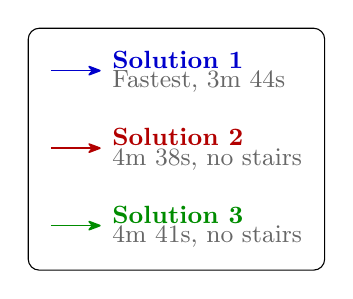
\begin{tikzpicture}[
    %% -- Node styles ------------------------------------------------------
    %%
    %% station: small pill/stadium shape used as the "dot" indicator.
    %%   The node body is EMPTY; the monospaced name lives OUTSIDE as a label.
    %%   Edges and positioning are anchored to the pill shape, not the text.
    %%
    %%   Usage:
    %%     \node[station, label={[stlabel]right:NODE\_ID}]               (A) {};
    %%     \node[station-bold, label={[stlabel-bold]right:NODE\_ID}]     (A) {};
    %%
    station/.style={
        draw,
        shape=rounded rectangle,   % from shapes.misc - true semi-circular ends
        rounded rectangle arc length=180,
        minimum height=0.9em,       % height sets the semicircle diameter
        minimum width=2.4em,        % must exceed height to get a flat middle section
        inner xsep=0pt,
        inner ysep=0pt,
        line width=1.6pt,
        fill=white,
    },
    %% station-bold + stlabel-bold: use on start/end/waypoint nodes for emphasis.
    station-bold/.style={station, line width=3pt},
    %% stlabel: monospaced name label placed to the right of the station dot.
    %%   Always pass it as the style argument to the label option:
    %%     label={[stlabel]right:NAME}
    stlabel/.style={font=\ttfamily, inner sep=2pt},
    stlabel-bold/.style={stlabel, font=\ttfamily\bfseries},
    %% -- Base directed edge style ------------------------------------------
    %%
    %%   All per-solution styles inherit from this.
    %%   For parallel edges use bend left/right:
    %%     \draw[sol1, bend left=20] (A) to node[elabel, above] {label} (B);
    route/.style={
        ->,
        >=Stealth[round],
        semithick,
        % shorten >=4pt,
        % shorten <=4pt,
    },
    %% -- Per-solution edge styles (one colour per solution) ----------------
    %%
    %%   Usage:  \draw[sol1] (A) -- (B);
    %%           \draw[sol2, bend left=20] (A) to node[elabel, above] {text} (B);
    sol1/.style={route, color=blue!80!black},           % Solution 1 - blue
    sol2/.style={route, color=red!70!black},            % Solution 2 - red
    sol3/.style={route, color=green!55!black},          % Solution 3 - green
    sol4/.style={route, color=orange!85!black},         % Solution 4 - orange
    sol5/.style={route, color=violet!80!black},         % Solution 5 - violet
    %% -- Edge label styles ------------------------------------------------
    %%
    %%   Use the per-solution variant (elabel1-elabel5) so that identical labels
    %%   on parallel edges are still distinguishable by colour.
    %%
    %%   For N parallel edges on the same node pair, spread them symmetrically:
    %%     N=2: bend left=15  /  bend right=15
    %%     N=3: bend left=25  /  straight (no bend)  /  bend right=25
    %%     N=4: bend left=35  /  bend left=12  /  bend right=12  /  bend right=35
    %%
    %%   To additionally separate labels, use xshift on the node option:
    %%     node[elabel3, right, xshift=8pt]
    %%
    %%   Example (2 parallel edges):
    %%     \draw[sol1, bend left=15]  (A) to node[elabel1, left]  {label} (B);
    %%     \draw[sol2, bend right=15] (A) to node[elabel2, right] {label} (B);
    %% -- Legend styles ------------------------------------------------------
    %%
    %%   legendtitle: bold coloured solution name - pair with the solution colour.
    %%     e.g. \node[legendtitle, text=blue!80!black] {Solution 1};
    legendtitle/.style={font=\small\bfseries, inner sep=0pt, anchor=west},
    %%   legenddesc: smaller grey text for the lines below the title.
    legenddesc/.style={font=\small, text=black!60, inner sep=0pt, anchor=west},
    elabel/.style ={font=\small\ttfamily, inner sep=5pt},
    elabel1/.style={elabel, text=blue!80!black},
    elabel2/.style={elabel, text=red!70!black},
    elabel3/.style={elabel, text=green!55!black},
    elabel4/.style={elabel, text=orange!85!black},
    elabel5/.style={elabel, text=violet!80!black},
]

%% -- Place nodes here -----------------------------------------------------

% omitted

%% -- Draw edges here ------------------------------------------------------

%% Solution 1 (blue):
% omitted

%% Solution 2 (red) - parallel to sol1 on shared segments, bent symmetrically:
% omitted

%% Solution 3 (green) - parallel to sol1 on shared segments, bent symmetrically:
% omitted

%% -- Legend --------------------------------------------------------------
%%
%%   Move the whole legend by changing the shift value.
%%   Each item occupies a vertical slot; the slot height is 2.8em.
%%   Copy/remove item blocks as needed and update the fit= list on the box node.
%%
%%   Item anatomy (all x-coordinates are relative to the scope origin):
%%     0        - arrow start
%%     1.8em    - arrow end / label start offset
%%     2.2em    - text column (title + description nodes)
%%     slot y   - 0, -2.8em, -5.6em, -8.4em, -11.2em  (for items 1-5)
%%
\begin{scope}[shift={(-6.5cm, -1cm)}]   %% change this to reposition the legend

    %% -- Item 1 --
    \node[inner sep=0, minimum size=0] (leg-orig) at (0, 0) {};  %% left-edge anchor
    \draw[sol1] (0, 0) -- (1.8em, 0);
    \node[legendtitle, text=blue!80!black]  (li1-title) at (2.2em,  0.4em) {Solution 1};
    \node[legenddesc]                       (li1-desc)  at (2.2em, -0.4em) {Fastest, 3m 44s};

    %% -- Item 2 --
    \draw[sol2] (0, -2.8em) -- (1.8em, -2.8em);
    \node[legendtitle, text=red!70!black]   (li2-title) at (2.2em, -2.8em+0.4em) {Solution 2};
    \node[legenddesc]                       (li2-desc)  at (2.2em, -2.8em-0.4em) {4m 38s, no stairs};

    %% -- Item 3 --
    \draw[sol3] (0, -5.6em) -- (1.8em, -5.6em);
    \node[legendtitle, text=green!55!black] (li3-title) at (2.2em, -5.6em+0.4em) {Solution 3};
    \node[legenddesc]                       (li3-desc)  at (2.2em, -5.6em-0.4em) {4m 41s, no stairs};

    %% -- Bounding box - update fit= when adding/removing items --
    \node[draw, rounded corners=4pt, inner sep=8pt,
          fit=(leg-orig)(li1-title)(li1-desc)(li2-title)(li2-desc)(li3-title)(li3-desc)
    ] {};

\end{scope}

\end{tikzpicture}
\end{document}